\documentclass[a4paper]{article}

\usepackage[utf8]{inputenc}
\usepackage[english]{babel}
\usepackage{fancyhdr,graphicx}
\usepackage[colorlinks=true,linkcolor=black,urlcolor=blue,bookmarksopen=true]{hyperref}

\newcommand{\materia}{[75.41] Taller de Programación I}
\newcommand{\trabajo}{Manual de proyecto}
\newcommand{\trabajoheader}{Ejercicio final }
\newcommand{\cuatri}{1c2019}
\newcommand{\cuatrimestre}{Primer cuatrimestre de 2019}
\newcommand{\grupo}{Grupo 3}

\newcommand{\autores}{
	Camila Bojman,
	Cecilia Hortas,
	Nicolas Vazquez}

\hypersetup{
	pdftitle={\trabajo},
	pdfsubject={\materia},
	pdfauthor={\autores},
}

\pagestyle{fancy}
\fancyhf{}
\fancyhead[L]{\materia}
\fancyhead[R]{\trabajoheader - \trabajo}
\renewcommand{\headrulewidth}{0.4pt}
\fancyfoot[C]{\thepage}
\renewcommand{\footrulewidth}{0.4pt}

\begin{document}
	\pagenumbering{gobble}
	\pagenumbering{roman}
	\pagenumbering{arabic}
	\setcounter{page}{1}
	
	\begin{titlepage}
		\hfill
\includegraphics[width=6cm]{fiuba.jpeg}
		\begin{center}
			\vfill
			\Huge \textbf{\trabajo}
			\vskip2cm
			\Large \materia\\
			\cuatrimestre
			\vfill
			\grupo
			\begin{itemize}
				\item Camila Bojman 101055 camiboj@gmail.com
				\item Cecilia Hortas 100687 ceci.hortas@gmail.com 
				\item Nicolas Vazquez 100338 vazquez.nicolas.daniel@gmail.com
			\end{itemize}
			\vskip1cm
		\end{center}
	\end{titlepage}

\section{División de tareas}

Para la división de tareas se eligió dividir el trabajo de una forma distinta a la dispuesta en el enunciado.
\begin{enumerate}
	\item Uno se encargó de realizar el cliente gráfico, implementado todo lo relativo a la interfaz gráfica del trabajo con el uso de la herramienta \texttt{SDL} y el soporte de la arquitectura cliente-servidor aplicando los conceptos vistos en la cursada de multithreading y sockets.
	\item Otro se encargó de realizar el servidor, modelando el juego desde su parte física con el uso de la libreria \texttt{Box2D} y el testing correspondiente con la librería \texttt{CxxTest}.
	\item Finalmente, el último integrante se encargó de realizar el editor de escenarios, con el uso de la herramienta \texttt{SDL} para graficar los elementos,  \texttt{ffmpeg} para brindar el soporte para la grabación de partidas y \texttt{yaml} para colocar en un archivo la información del escenario.
\end{enumerate}

\section{Evolución del proyecto}
El cronograma propuesto por la cátedra pudo seguirse en las primeras semanas de resolución, no así las últimas semanas. Se consideró que hubo un aumento abrupto de tareas en la transición de la semana 3 a la semana 4, lo cual causó un atraso que fue reproduciendóse en el transcurso de las siguientes semanas. El soporte físico del juego se consideró finalizado 1 semana antes de la fecha de entrega final y el cliente gráfico 1 semana antes, lo cual significó que el soporte de sockets y multithreading se desarrolló en las últimas 2 semanas del trabajo, cuando lo previsto era empezarlo 2 semanas antes. En cuanto al editor, sucedió algo similar debido a que la finalización del mismo se concluyó 1 semana antes y lo esperado era algunas semanas atrás. 

\section{Inconvenientes encontrados}
En cuanto al servidor, un gran inconveniente encontrado fue relativo a la librería \texttt{Box 2D}. Si bien la misma está muy bien documentada y se encuentra un amplio material sobre ello en internet, algunos elementos no son amigables para su implementación e interpone algunas dificultades. Así mismo, en lo personal algunos detalles de implementación que propone la librería resultan contrarias a la filosofía de programación orientada a objetos que se espera obtener con el trabajo, por lo que implicó un gran tiempo empleado en un diseño relativamente compatible con ella. Otro factor a tener en cuenta es que la amplia variedad de funcionalidades que se espera obtener del juego puede resultar un trabajo bastante pesado para la cantidad de tiempo estipulado y genera muchos casos borde que pueden ser dificiles de alcanzar y sobretodo debuggear en un trabajo de este nivel.

En el editor, como en cualquier proyecto, la primera traba se dio durante la interiorización de su librería principal SDL. Una vez pasada esta barrera el editor siguió su rumbo a muy buen ritmo hasta toparse con la implementación de las compuertas lógicas.
Las compuertas lógicas atrajeron dos problemas. En primer lugar la necesidad de volver a interiorizarse con otra librería (también de SDL) para poder interactuar con el usuario. Para ello se quería escribir un mensaje en pantalla para informar al usuario lo que había que hacer. A su vez se quería recibir la respuesta que ingrese el usuario (mostrando también este por pantalla).  En segundo lugar el modelo planteado no había tenido en cuenta este feature. Llegar al modelo final conllevó mucho tiempo de planeamiento, varias refactorizaciones, bugs y aún así sentimos que la implementación no es la más prolija/clara. No obstante, creemos que vale la pena aclarar que la primera dificultad fue menor en comparación a la dificultad de plantear un modelo que realmente se adapte a este feature.
Por último un inconveniente mínimo generado por la librería gráfica fue el acarreo de dependencias. Se decidió simplemente arrastrar esto durante todo el trabajo ya que el origen de este inconveniente no era nuestro.

Finalmente, en cuanto al cliente los principales problemas surgieron de realizar las clases que simulan ser un wrapper de las funcionalidades de dibujo de SDL. Además presentó una dificultad adicional modelar la arquitectura cliente-servidor y manejar de manera adecuada los threads para no caer en problemas de concurrencia.


\section{Análisis de puntos pendientes}

En cuanto al modelo de juego no se llegó a implementar los portales sobre los bloques diagonales y la muerte de Chell al cerrar una compuerta. Además se podrían pulir más los valores de las fuerzas y velocidades utilizados para darle un enfoque más realista al juego. Por ejemplo hubiese estado bueno modelar la toma de la roca de una manera en la cual se pueda hacer clic en la misma y Chell la transporte además de que sea posible poder saltar con ella. Esto no pudo realizarse en un primer lugar por falta de tiempo y en un segundo lugar por el protocolo planteado de comunicación entre cliente y servidor, ya que hacer clic en una piedra implicaba un factor de error en el cálculo de los centros de masa y se consideró que empeoraba la performance al tener que ser una búsqueda lineal sobre las mismas. 

El editor si bien cumple con lo pedido en la consigna hay pequeñas mejoras pendientes. Los objetos más grandes, como por ejemplo los bloques de metal, son interpretados por el modelo como un objeto real y luego centinelas que completan el tamaño necesario. En nuestro ejemplo, el bloque de metal que vemos al usar el editor está dividido en cuatro partes iguales.

\begin{figure}[!h]
	\makebox[\textwidth][c]{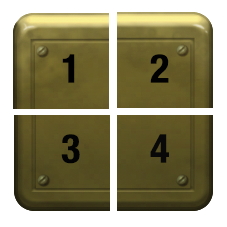
\includegraphics[width=0.25\textwidth]{mb_editor.png}}
	\caption{Un bloque en el editor}
	\label{fig:diagrama1}
\end{figure}

La esquina inferior izquierda es realmente un bloque de metal y las otras 3 esquinas son simplemente centinelas que el editor guarda para saber que la posición está ocupada (en este caso ocupada por el bloque de metal pero el modelo no sabe esto). El problema es que esta forma de implementar el editor no logró ser completamente transparente al usuario. Si el usuario cliquea un bloque de metal sobre alguna de las 3 esquinas-centinelas no obtendrá ninguna respuesta. Solucionar este problema pensamos que no requiere de mucho trabajo pero a la hora de priorizar las tareas debido al tiempo que quedaba no terminó en una buena posición. 
Otro feature que quedó pendiente fue poder abrir un escenario en cualquier momento de la edición, no sólo en una primera instancia. Esta idea tenía una dificultad menor a la anterior pero también una prioridad.
Las últimas dos ideas que quedaron pendientes fueron agregarle musica al editor y que los objetos seleccionados queden seleccionados una vez colocados en el escenario. Es decir que cuando el usuario seleccione un bloque de metal del menú luego pueda poner la cantidad de bloques que quiera en el escenario teniendo que acceder al menú sólo si quiere colocar un objeto distinto.

Finalmente, en cuanto a la arquitectura cliente-servidor se considera que faltaría incluir soporte para reconectar un cliente al terminar una partida, mostrar los jugadores conectados a una partida y cuánto falta para llenar el juego. En el cliente faltaría implementar un sistema de sonido con una mayor variedad de sonidos, además de incluir una transición entre temas en el medio del juego. Sin ir más lejos, la animación relativa al motor gráfico podría ser mejorada para soportar una mejor transición entre animaciones.

\section{Herramientas}

Las herramientas utilizadas para el desarrollo del trabajo, además de las mencionadas que son obligatorias en la resolución son las que siguen:

\begin{itemize}
	\item \texttt{IDE Clion}
\end{itemize}

Ofreció un gran apoyo para el desarrollo general del trabajo. Su herramienta de debugger fue especialmente útil así como el compilador \texttt{CMake} que ofrece, permitiendo agilizar enormemente el proceso de debuggeo y compilación.

\begin{itemize}
	\item \texttt{Git}
\end{itemize}

Se utilizó como herramienta de control de versiones, permitiendo el desarrollo individual de cada parte del trabajo de una forma organizada y segura.

\begin{itemize}
	\item \texttt{Latex} 
\end{itemize} 

Se utilizó para escribir la documentación y los manuales requeridos por el trabajo.

\section{Conclusiones}

A modo de conclusión se puede afirmar que el objetivo fue cumplido a grandes rasgos y que constituyó una gran experiencia de aprendizaje. Igualmente cabe mencionar que los objetivos planteados son bastantes para la cantidad de semanas estipulada, aunque no podría haber una alternativa frente al tiempo necesario para adquirir los conceptos a emplear.

\end{document}